\documentclass[10pt]{article}
\usepackage{fullpage}
\usepackage[pdftex]{graphicx}
\usepackage{rotating}
\usepackage{multirow}
\usepackage{subfigure}
\usepackage{url}
\usepackage{amsmath}
\usepackage{amssymb}
\usepackage{wasysym}
\usepackage{algorithm}
\usepackage{algpseudocode}

\newcommand{\etal}{\emph{et al.}}

\setlength\parindent{0pt} % sets indent to zero
%\setlength{\parskip}{10pt}

\begin{document}
\title{$k$-Nearest Neighbour Search Using Space-filling Curves}
\author{Camara Lerner \hspace{2cm} Christopher Rabl \\
  Department of Mathematics and Computer Science \\
  University of Lethbridge, Canada}

\maketitle

\section{Introduction}

In the field of Machine Learning, the $k$-nearest neighbour problem is defined as follows: we are given a set of points $P = \left\{ {(v_i, c_i) : v_i \in \mathbb{R}^d, c_i \in C } \right\}$, where $C$ is a set of class labels (for instance, a binary class labeling would be: $C = \left\{ {0,1} \right\}$) and $v_i$ is a $d$-dimensional vector. The task at hand is, given a point $(q, c) \not \in P$, and where $c$ is unknown, attempt to assign a class label from $C$ the point based on the values of the $k$ closest vectors to $q$ in $P$. In this paper, we will attempt to simply perform the latter task: determine which $k$ points in $P$ are approximately the closest to a given query point. \\

Our implementation will be stated as an appoximation algorithm, since all methods of calculating kNN exactly are marred by the so-called ``curse of dimensionality'' \cite{Bellman:2003}. Even though it is not an NP-Complete problem, it is still difficult to calculate kNN in high dimensions since, if we assume that the algorithm is acting on $n$ $d$-dimensional points, the naive implementation takes $O(dn)$ time. Approaches such as spatially-ordered trees (such as quadtrees and $kd$-trees) and space-filling curves have been applied to this problem in order to approximate it more quickly than the naive approach (calculating a distance matrix between each point and choosing the smallest $k$ non-zero entries from the row corresponding to the query point). \\

This particular approach utilizes the unique properties of space-filling curves in order to achieve its goal. In this paper, we will detail our method, detail a software implementation of these algorithms, and produce experimental data in order to determine which curve yields the most satisfactory approximation to the problem. Contrary to the original project proposal, the authors decided against exploring the approach of Dahl and Wootters \cite{Dahl:2008} due to a significant lack of implementation specificity: many important details were completely omitted from the paper and could not be extrapolated based on the context of the statements in which they appeared. Instead, a variant of method by Connor and Kumar \cite{Connor:2010} was chosen, since comparing and contrasting the neighbourhood-preserving properties of each space-filling curve turned out to be a more fruitful and unique comparison.

\section{Space-Filling Curves}

From a general standpoint, a space-filling curve is a mapping $M : \left\{ {1 ... n} \right\}^d \rightarrow \left\{ {1 ... n^d} \right\}$ which induces a 1-dimensional ordering on a set of points in $d$-dimensional space \cite{Bader:2013}. However, the utility of these curves comes not from this mapping but from a property called ``locality preservation'' which centers on the notion that points which are close together in the input space should be close to each other on the space-filling curve. While this ideal is not necessarily achieved in every instance (especially in higher dimensions), it provides a reasonably effective way of retrieving a list of ``candidate'' nearest-neighbours. Moreover, it is possible to compute the results of this mapping within a reasonably quick amount of time ($O(d)$ in the case of Morton ordering) and therefore is a solid foundation upon which an approximation algorithm may be built.

\section{Morton Ordering}

Calculating the Morton order (or Z-order as it is commonly called) of a given point in $d$ dimensions is a fairly straightforward process, and can be done on an arbitrarily large list of points to create a Morton ordering. This particular ordering features prominently in the approach taken by Connor and Kumar \cite{Connor:2010}, and the implementation of their functions {\bf COMPARE} (used to compare the Morton order of two points) and {\bf FirstMSB} (which calculate the index of the smallest most-significant bit between two bit strings) are detailed below. In Algorithm~\ref{first-msb}, the $\mathrel{\&}$ operator represents the bitwise-AND operation.

\begin{algorithm}
  \caption{COMPARE(point ${\bf p}$, point ${\bf q}$)}
  \label{compare}
  \begin{algorithmic}[1]
    \State $x \leftarrow 0, dim \leftarrow 0$
    \ForAll{j=0 to d}
    \State $y \leftarrow \text{FirstMSB}(p_{[j]}, q_{[j]})$
    \If{$x < y$}
    \State $x \leftarrow y, dim \leftarrow j$
    \EndIf 
    \EndFor \\
    \Return $p_{[dim]} < q_{[dim]}$
  \end{algorithmic}
\end{algorithm}

\begin{algorithm}
  \caption{FirstMSB(double $a$, double $b$)}
  \label{first-msb}
  \begin{algorithmic}[1]
    \State $w \leftarrow x < y \text{ and } x < (x \mathrel{\&} y)$ \\
    \Return $w$
  \end{algorithmic}
\end{algorithm}

\section{Hilbert Curve}

A Hilbert curve of order $m$ is a space-filling curve that is based on a generalization of Gray codes in $n$ dimensions. In turn, it may be used to fill a space whose axis points are within the range $\left\{{1...2^m}\right\}$. This means that for each point in the curve, the number of bits required to represent the Hilbert order is $(mn)$. The algorithm used in our implementation is adapted from~\cite{Hamilton:2006}. \\

The curve labels the points from $0$ to $2^{mn} - 1$ in the order that the curve visits each point. The Hilbert Curve considered here begins at the origin. We call the Hilbert curve of order 1 the unit Hilbert curve: as the order increases, this basic curve is reflected and rotated and moved around to fill the space of the larger Hilbert Curve, and then these unit Hilbert curves are connected to make the overall Hilbert curve. The only constraint on the unit Hilbert curve is that the start and end points must match up with their neighbouring unit Hilbert curves.

\flushleft
The formula for calculating the Gray code can be found in~\ref{gray-code}.
\begin{equation}
  \label{gray-code}
  gc(i) = i \oplus \left( i \gg 1 \right) 
\end{equation}

\begin{algorithm}
  \caption{The algorithm for calculating the Gray Code Inverse $(gc^{-1}(g))$ of $g \in \mathbb{N}$, calculates the $i \in \mathbb{N}$ such that $gc\left( i \right) = g $ }
  \label{gray-code-inverse}
  \begin{algorithmic}[1]
    \Require $g \in \mathbb{N}$ 
    \State $ m \leftarrow \text{ number of bits to represent } g$ 
    \State $ \left( i, j \right) \leftarrow \left( g, 1 \right) $ 
    \While{$ j < m $ }
    \State $ i \leftarrow i \oplus \left( g \gg j \right)$ 
    \State $ j \leftarrow j + 1$ 
    \EndWhile \\
    \Return $i$ % \in \mathbb{N} \text{ such that } gc \left( i \right) = g $
  \end{algorithmic}
\end{algorithm}

In order to calculate the next point in the Hilbert ordering, we must find its Gray code value, which may be done using~(\ref{g}).
\begin{equation}
  \label{g}
  g(i) = \lfloor \log _{2} \left( gc(i) \oplus gc(i+1) \right) \rfloor + 1
\end{equation}


The direction of the unit Hilbert curve in each iteration is calculated by~(\ref{d}).
\begin{equation}
  \label{d}
  d(i) = 
    \begin{cases}
      0 & \quad \text{if $i = 0$}\\
      g(i - 1) \pmod{n} & \quad \text{if $i$ is even} \\
      g(i) \pmod{n} & \quad \text{if $i$ is odd}
    \end{cases}
\end{equation}

The entry point of the unit Hilbert curve in each iteration is calculated by~(\ref{e}).
\begin{equation}
  \label{e}
  e(i) =  
    \begin{cases}
      0 & \quad \text{if $i = 0$}\\
      gc(2 * \lfloor x-1/2 \rfloor) & \quad \text{otherwise} \\
    \end{cases}
\end{equation}

Formula for the bitwise right rotation is displayed in~(\ref{right-rotate}). The bitwise left rotation is similar.
\begin{equation}
  \label{right-rotate}
  a \rightturn i = \left[ a_{{n - 1 + i}\pmod{n}} \ldots a_{i\pmod{n}} \right]_{\left[ 2 \right]}, \text{ where } a = \left[ a_{n-1} \ldots a_0\right]_{\left[ 2 \right]} 
\end{equation}

In determining the Hilbert curve index, the $l$ variable used in~(\ref{hilbert-point-to-index}) has each bit representing whether the point is above or below the axis corresponding to each bit. The $e$ and $d$ variables represent the rotations and reflections nessesary to map the current sub-Hilbert curve containing the point ${\bf p}$ to the normal orientation of sub-Hilbert curve. These values are recalculated until the sub-Hilbert curve is a unit Hilbert curve. There is also a variable $w$, which is calculated at every iteration that is OR-ed with $h$ after $h$ is bit-shifted left one bit. Then, after all the iterations $h$ is the index of the point ${\bf p}$. This algorithn runs in $O(m^2)$ time.

\begin{algorithm}[H]
  \caption{Calculates the Hilbert index given any dimensional point ${\bf p}$ 
    of size $n$ as long as the bits used within an index of the hilbert curve 
    space is specified in ($m$).}
  \label{hilbert-point-to-index}
  \begin{algorithmic}[1]
    \Require $n, m \in \mathbb{N} - \{0\} \text{ and a point } {\bf p} \in \mathbb{N}^n$ 
    \State $ \left( h, e, d \right) \leftarrow \left( 0, 0, 0 \right) $
    \For{$j\gets m - 1, 0$} 
    \State $ l \leftarrow \left[ \left( p_{n-1} , i \right) \ldots \left( p_0 , i \right) \right]_{\left[ 2 \right]} $ 
    \State $ l \leftarrow \left( l \oplus e \right) \rightturn \left( d+1 \right)$ 
    \State $ w \leftarrow gc^{-1} \left( l \right)$ 
    \State $ e \leftarrow e \oplus \left( e \left( w \right) \leftturn \left( d+ 1 \right) \right) $ 
    \State $ d \leftarrow d + d \left( w \right) + 1 \pmod{n}$ 
    \State $ h \leftarrow \left( h \ll n \right) | w $
    \EndFor \\
    \Return $h $%\in \mathbb{N} \text{, the Hilbert index of the point }{\bf p}$

  \end{algorithmic}
\end{algorithm}

\section{Constructing kNN Sets}

The algorithm of Connor and Kumar \cite{Connor:2010} begins by inducing a Morton order on a set of $n$ points (called $P$) in $d$ dimensional space. We have extended this set construction algorithm to also induce a Hilbert order on the same set of points. Both of these orderings are accomplished using special comparison operators which take two vectors and compute their relative ordering on the given space-filling curve. Using QuickSort and these operators, it is possible to perform this ordering step in $O(n \log{n})$ time. \\[10pt]

\begin{algorithm}[H]
  \caption{kNN Set Construction Algorithm}
  \label{knn-graph-alg}
  \begin{algorithmic}[1]
    \Require $\text{Morton order comparison operator: } < 
    \text{ and Hilbert order compare operator: } <$
    \Ensure $A_i \text{ contains } k \text{ nearest neighbors of } p_i \text{ in } P \text{.}$
    \State $P \leftarrow \text{QuickSort}(P, <)$
    \ForAll{$p_i$ in $P$}
    \State $A_i \leftarrow \text{SET-KNN}(p_i, \{p_{i-k}, \dots, p_{i+k} \})$
    \If{$\text{SHIFT}(p_i, \lceil \text{SET-RAD}(A_i) \rceil) < p_{i+k}$}
    \State $upper \leftarrow i$
    \Else
    \State $I \leftarrow 1$
    \While{$\text{SHIFT}(p_i, \lceil \text{SET-RAD}(A_i) \rceil) < p_{i+2^I}$}
    \State $++I$
    \EndWhile
    \State $upper \leftarrow \text{min}(i+2^I, n)$
    \EndIf
    \If{$\text{SHIFT}(p_i, - \lceil \text{SET-RAD}(A_i) \rceil) > p_{i-k}$}
    \State $lower \leftarrow i$
    \Else
    \State $I \leftarrow 1$
    \While{$\text{SHIFT}(p_i, - \lceil \text{SET-RAD}(A_i) \rceil)$}
    \State $++I$
    \EndWhile
    \State $lower \leftarrow \text{max}(i-2^I, 1)$
    \EndIf
    \If{$lower \not= upper$}
    \State $A_i \leftarrow \text{CSEARCH}(p_i, lower, upper)$
    \EndIf
    \EndFor \\
    \Return $A_i$
  \end{algorithmic}
\end{algorithm}

Next, for each point $p_i \in P$, a partial solution $A_i$ is found by performing a linear search of the $2k$ nearest neighbors to $p_i$ in the given ordering. This is done using the naive kNN search method (called {\bf SET-KNN} in Algorithm~\ref{knn-graph-alg}) which has a complexity of $O(kd)$. In order to yield a better partial solution, we shift the bounds of the linear search window. This is done using the {\bf SHIFT}($p$, $s$) operation which adds $s$ units to every component of point $p$. In order to find satisfactory upper and lower bounds on this search window, a measure called {\bf SET-RAD} is used: {\bf SET-RAD}($S$) returns the maximum distance between any two points in a set $S$. \\[10pt]

Once the search window is exhausted, a function called {\bf CSEARCH} performs a binary search within the partial solution window in order to find the closest neighbours to $p_i$ within the window. This search is only done if the size of the resulting window is non-zero. Finally, the set $A_i$ is returned, which contains the approximate $k$ nearest neighbours to $p_i$ in $P$. \\[10pt]

Within the {\bf CSEARCH} function there is $v$, a platform-specific constant which, according to \cite{Connor:2010} was found to be 4, as well as {\bf CIRCLE}($c$, $r$) which computes the coordinates of the circumference of a circle centered at $c$ and that has radius $r$. {\bf DIST}($a$, $b$) denotes the Euclidean distance between two points $a$ and $b$ in $d$ dimensions. Since {\bf CSEARCH} uses a form of binary search, its running time is bounded by $O(\log{n})$.

\begin{algorithm}[H]
  \caption{CSEARCH(point $p_i$, int $lo$, int $hi$)}
  \label{csearch}
  \begin{algorithmic}[1]
    \If{$(hi - lo) < v $}
    \State $A_i \leftarrow \text{SET-KNN}(p_i, A_i \cup \{ p_{lo} \dots p_{hi} \})$
    \Return $A_i$
    \EndIf
    \State $mid \leftarrow (hi+lo)/2$
    \State $A_i \leftarrow \text{SET-KNN}(p_i, A_i \cup p_{mid})$
    \If{$\text{DIST}(p_i, \text{CIRCLE}(p_{lo}, p_{hi})) \ge \text{SET-RAD}(A_i)$} 
    \Return $A_i$
    \EndIf
    \If{$p_i < p_{mid}$}
    \State $A_i \leftarrow \text{CSEARCH}(p_i, lo, mid-1)$
    \If{$p_{mid} < \text{SHIFT}(p_i, \lceil \text{SET-RAD}(A_i) \rceil)$}
    \State $A_i \leftarrow \text{CSEARCH}(p_i, mid+1, hi)$
    \EndIf
    \Else
    \State $A_i \leftarrow \text{CSEARCH}(p_i, mid+1, hi)$
    \If{$\text{SHIFT}(p_i, - \lceil \text{SET-RAD}(A_i) \rceil) < p_{mid}$}
    \State $A_i \leftarrow \text{CSEARCH}(p_i, low, mid - 1)$
    \EndIf
    \EndIf \\
    \Return $A_i$
    
  \end{algorithmic}
\end{algorithm}

\section{Implementation Correctness}

In order to ensure the correctness of our implementation, some small test cases were generated and verified by hand over the course of the development process. These were computed manually but implemented in the form of Python unit tests using the UnitTest library. Additionally, the correctness of the ordering operators were verified using a similar approach. \\[10pt]

Experimental data was generated both randomly and deterministically in order to test the efficiency and effectiveness of the algorithms: real-world datasets were also obtained and evaluated as part of our experiment, specifically the ``Yeast times 100'' dataset which consists of 1484 vectors in 8 dimensions, and the ``ARCENE'' dataset \cite{ARCENE:2004} which consists of 700 vectors in 1024 dimensions. Both real-world datasets were obtained from the UCI Machine Learning Repository \cite{UCI:2013}. \\[10pt]

These datasets were used to assess the performance of the different space-filling curve methods on high- and very high-dimensional real-world data. All experimental results were collected using Python 2.7.5 on Mac OS X 10.9. The system configuration used to test the algorithm was a mid-2013 Apple MacBook Air with a 1.3GHz Intel Core i5 processor and 4GB of RAM.

\section{Experiment}

Since an integer lattice point in $d$ dimensions will have $2d$ nearest neighbours, rather than examining the lists returned by the $2d$-nearest neighbour function and comparing them, we devised a metric called ``average SET-RAD ratio'', which is defined in Equation~\ref{avg-set-rad}. OPT[$i$] in this case was calculated by the naive method (SET-KNN on the entire set) and provided an a-posteriori guarantee on solution quality. We chose this measure since it provided a bound on the algorithm’s worst result in every case (since {\bf SET-RAD} gives the maximum distance between any pair points in a set). This is taken as an average over all iterations of the algorithm’s main loop. 

\begin{equation}
  \label{avg-set-rad}
  \frac{1}{n} \sum_{i=1}^n \frac{\text{SET-RAD}(A_{AKNN}[i])}{\text{SET-RAD}(A_{OPT}[i])}
\end{equation}

A running time analysis was also performed in order to determine whether the type of space-filling curve used in the algorithm had any effect on its running time.

\section{Results}

As evidenced in the figures~\ref{run-yeast},~\ref{run-arcene}, and~\ref{run-lattice}, we see that the algorithm has a roughly sub-quadratic running time. This is an asset when dealing with high-dimensional data sets such as ARCENE, but comes as a detriment when smaller sets (such as the ``lattice'' dataset) are used. Impressively, in the case of the ARCENE dataset ($d = 1024$, $n = 700$), when $k=4$ the algorithm using Morton ordering was more than 7 times faster than the naive approach. \\[10pt]

In terms of a bound on solution quality, using the metric in Equation~\ref{avg-set-rad}, we have determined an approximation factor of around $\alpha=1.3$ for Morton AKNN, and $\alpha=1.2$ for Hilbert AKNN. Due to the solution quality metric being used, however, these values should not be considered rigorous bounds, as they have not been rigorously proven.

\section{Conclusion}

In this paper, we have outlined and tested a method to calculate the $k$ nearest neighbours of a point in $d$ dimensions. Through our analysis, we have shown that by inducing a space-filling curve on the set of points, and using some search operations, we were able to obtain an approximate solution in a relatively short amount of time for small values of $k$. Our implementation lags behind the naive method when confronted with sets of points in low dimensions, but works well when tested on high-dimensional sets. Finally, we have shown that by utilizing the Hilbert space-filling curve, we are able to obtain a tighter approximation of the solution for most values of $k$ at the cost of a slightly longer running time.


\begin{figure}
\begin{center}
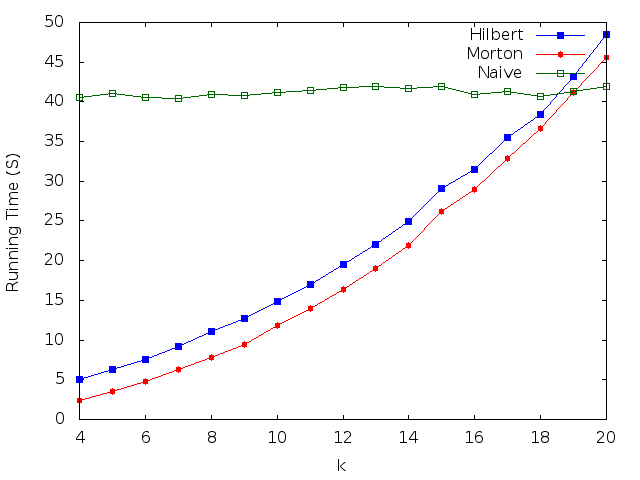
\includegraphics[scale=0.5]{YeaGra.png}
\caption{Running time analysis of the Yeast dataset ($d = 8$, $n = 1484$), lower is better.}
\label{run-yeast}
\par\vspace{\intextsep}
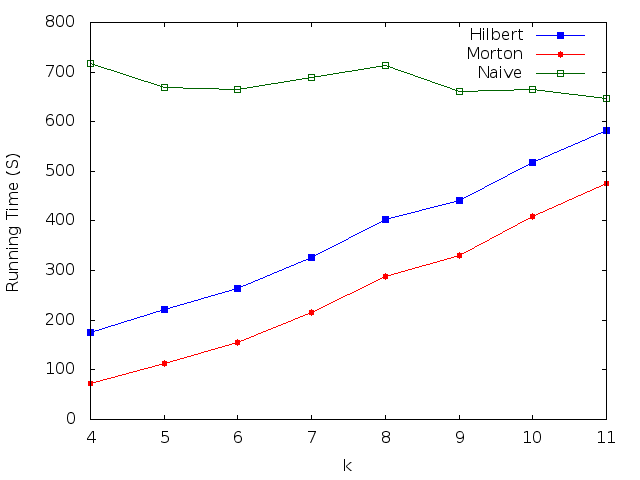
\includegraphics[scale=0.5]{ArcGra.png}
\caption{Running time analysis of the ARCENE dataset ($d = 1024$, $n = 700$), lower is better.}
\label{run-arcene}
\end{center}
\end{figure}

\begin{figure}
\begin{center}
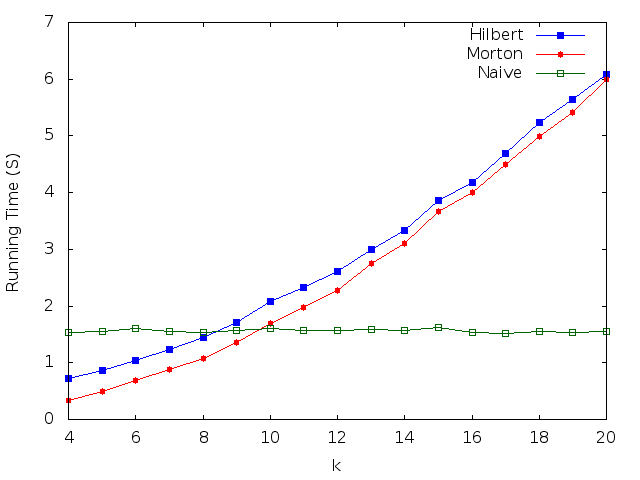
\includegraphics[scale=0.5]{LatGra.png}
\caption{Running time analysis of the integer lattice dataset ($d = 2$, $n = 1600$), lower is better.}
\label{run-lattice}
\end{center}
\end{figure}

\begin{figure}
\begin{center}
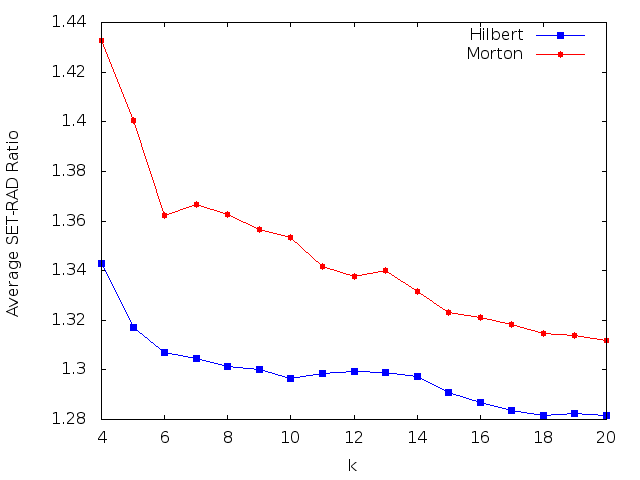
\includegraphics[scale=0.5]{YeaGra2.png}
\caption{Approximation bound of the Yeast dataset ($d = 8$, $n = 1484$), lower is better.}
\label{approx-yeast}
\end{center}
\end{figure}

\begin{figure}
\begin{center}
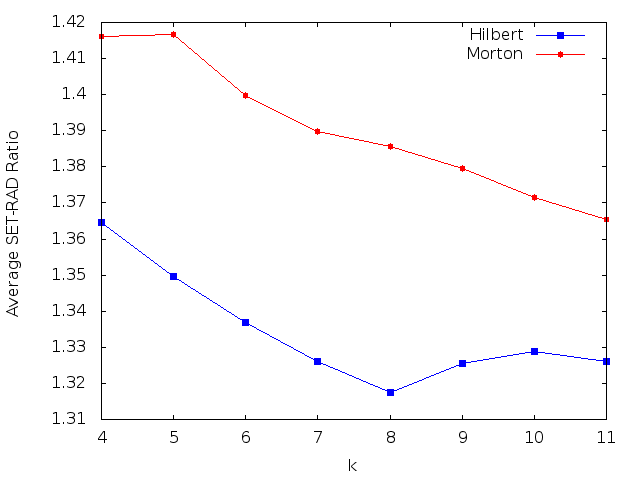
\includegraphics[scale=0.5]{ArcGra2.png}
\caption{Approximation bound of the ARCENE dataset ($d = 1024$, $n = 700$), lower is better.}
\label{approx-acrene}
\end{center}
\end{figure}

\begin{figure}
\begin{center}
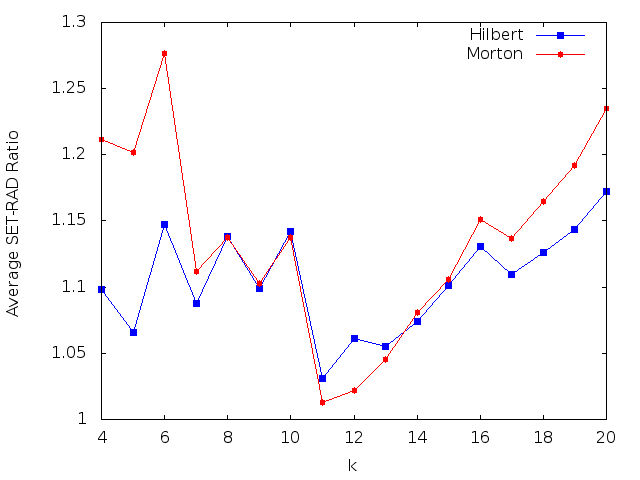
\includegraphics[scale=0.5]{LatGra2.png}
\caption{Approximation bound of the integer lattice dataset ($d = 2$, $n = 1600$), lower is better.}
\label{approx-lattice}
\end{center}
\end{figure}

\bibliographystyle{amsplain}
\bibliography{mybiblio}

\end{document}

